\documentclass{customization}

\usepackage{multicol}
\usepackage{comment}
\usepackage{textcomp}
\usepackage{xcolor}
\usepackage{calc}

\usepackage{listings}
\usepackage[most]{tcolorbox}
\usepackage{inconsolata}

% Code listing setup
\lstset{showstringspaces=false}
\definecolor{logocolor}{rgb}{0.11, 0.19, 0.33}
\newtcblisting[auto counter]{sexylisting}[2][]{sharp corners, 
    fonttitle=\bfseries, colframe=logocolor, listing only, 
    listing options={basicstyle=\ttfamily,language=java}, 
    title=Code example \thetcbcounter: #2, #1}


\title{Summer Student Project Report}

\begin{document}


%------------ Information ---------------------

\titre{A data-driven approach \\ to configure permanent tasks
\\ in LHCb Online farm}
\UE{LHCb Online}
\sujet{\LaTeX Blabla}

\enseignant{\underline{Markus \textsc{Frank}}\\
			\underline{Beat \textsc{Jost}}}

\eleves{\href{https://www.linkedin.com/in/3sztof/}{\underline{Krzysztof \textsc{Wilczyński}}}}

%----------- Initialization -------------------
        
\fairemarges 
\fairepagedegarde 

\begin{Large}
\centerline{\textbf{Abstract}}
\end{Large}
\vspace{0.5cm}

%==============================================
%               Abstract
%==============================================


During the boot sequence, the LHCb Online system consisting of about 1700 CPUs needs to configure roughly 2 dozen different types of standard, off the shelf processor units, each running a dedicated set of permanent processes. In this report, a data driven approach is presented where these node types and the corresponding processes are modeled using a relational database.
\newline

\noindent
Starting from the database model, a set of utility applications were derived. These include a command line interface, a web based graphical user interface and a program to verify the existence of the processes on a given node. Future extensions can easily be implemented using the provided application programming interface. 



% Old abstract (before the edit by Markus)
\begin{comment}
In the current LHCb Online farm process controller, all of the permanent task configurations are formed by a single, large and increasingly difficult to maintain Python script. Therefore, any change to the configuration or expansion of the system is made by labor-intensive edits of the code. The configuration is currently fairly complex and it would only get more confusing with the expansion of the farm in the future.
\newline

\noindent
To overcome the deficiencies of the present solution and to have a single source of information about the processes that should execute on a given node, the idea of developing a database-driven, flexible and expandable system emerged. 
\end{comment}


\tabledematieres  % Contents

%---------------- Body ------------------------


%==============================================
%               Introduction
%==============================================

\section{Introduction} 
\hspace{0.6cm}

As a part of LHCb Online group activities, the project had purely applied nature. It could be classified as full-stack IT development, from database back-end, trough application programming interface and unit testing, to command line and graphical user interfaces. There was some time scheduled for experiments and technology / protocol comparison that was very enriching for the author - a Summer Student.
\newline

\noindent
This document aims to give a brief description of the project, without going into technicalities. Implementation details allowing to recreate, explore and diagnose the solution's source code were described in the Appendix section of this document, should the reader be interested in more in-depth information.

\begin{comment}
\newline
\noindent\fcolorbox{logocolor}{white}{%
    \parbox{\textwidth}{%
        \centering
        \href{https://bitbucket.org/3sztof/lhcb_online/src/master/Docs/Project_Report/Summer_Student_Project_Technical_Report.pdf}{Summer Student Project Technical Report (LINK)} 
    }%
}
\end{comment}


%==============================================

\subsection{Online farm nodes and permanent tasks}
\hspace{0.6cm}

An online farm is a cluster of multipurpose computing machines (also referred to as: CPUs, nodes) that are grouped according to their purpose: high level triggering, online analysis of data, storage, logging, monitoring et cetera. An outlook of LHCb Online farm architecture is shown in figure \ref{fig:farm}.

\begin{figure}[H]
    \centering
    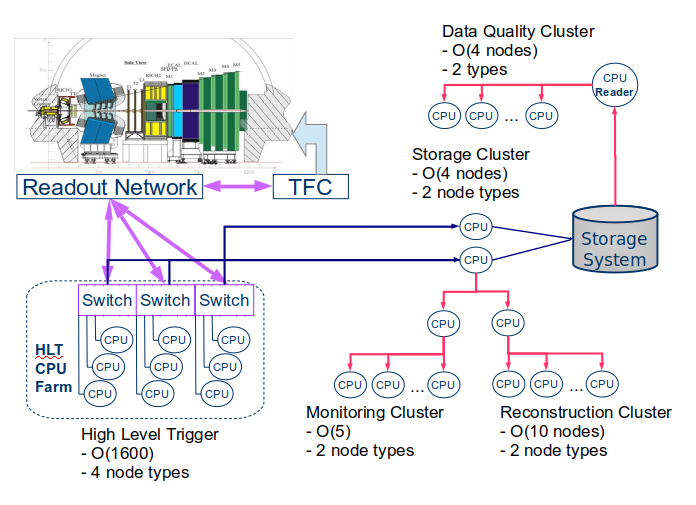
\includegraphics[scale=0.5]{images/farm.png}
    \caption{The LHCb Online farm architecture}
    \label{fig:farm}
\end{figure}

%==============================================

\noindent
The node groups such as "High Level Trigger" or "Reconstruction Cluster" shown in figure \ref{fig:farm} are defined by sets of permanent tasks (processes) running on each node in the given group. Those processes are started on the nodes at system boot and continue to run during the entire operation time (unlike special tasks that may be started and stopped anytime).
\newline

\noindent
An artificial hierarchy of tasks, task sets, node classes and nodes (top level regular expressions) emerged as a way of imagining and documenting the complex relations between the purpose of node groups and the tasks running on them. A diagram shown in figure \ref{fig:hierarchy} describes the parent-child relation between those groups. This hierarchical structure proved itself to be useful in the current solution and was not changed during the project. The main goal was to make the access to the underlying configuration data easier (more details on the aims of the project can be found in section 2).

\begin{figure}[H]
    \centering
    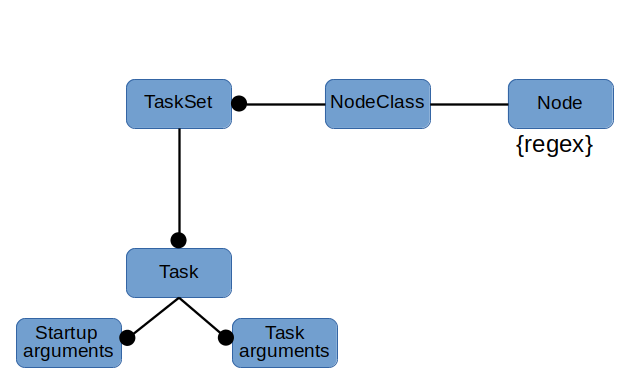
\includegraphics[scale=0.45]{images/hierarchy.png}
    \caption{The task hierarchy in the farm}
    \label{fig:hierarchy}
\end{figure}

%==============================================

\subsection{Online farm process controller}
\hspace{0.6cm}

The process controller is a part of LHCb FMC (Farm Monitoring and Control System) that is responsible for starting, stopping and maintaining the processes running on worker nodes in the online farm.
\newline

\noindent
Special nodes - "control PCs" are hosts of "pcSrv" process that allows them to supervise processes running on worker nodes assigned to them (each control PC in the current system oversees up to 32 nodes).
\newline

\noindent
The above description can be perceived as over-simplified. To find more details about the process controller and underlying DIM (Distributed Information Management system) services, please consult the Researchgate article by Federico Bonifazi, Daniela Bortolotti, Angelo Carbone, Domenico Galli, Daniele Gregori, Umberto Marconi, Gianluca Peco and Vincenzo M. Vagnoni linked below.
\newline 

\noindent\fcolorbox{logocolor}{white}{%
    \parbox{\textwidth}{%
        \centering
        \href{https://www.researchgate.net/publication/268357086_The_Process_Controller_for_the_LHCb_On-Line_Farm_Prepared_by}{The Process Controller for the LHCb Online Farm (LINK)}. 
    }%
}
    
%==============================================
%               Motivation
%==============================================

\newpage
\section{Motivation}
\hspace{0.6cm}

This section clarifies (hopefully) the reasons behind the development of a new system for permanent tasks configuration in LHCb online farm.

%==============================================

\subsection{Farm boot script}
\hspace{0.6cm}

Up to this point, all processes started on the farm nodes and their configuration data (parameters) were grouped in a single, large (and increasingly difficult to maintain) python script that prints out ready to execute "pcAdd" commands for a given node name. Those commands are then executed by the control PCs - the tasks are started on the nodes specified by their name (or a regular expression pointing to a group of nodes).
\newline

\noindent
Here is a simplified structure of a pcAdd command (pseudocode):
\newline

\begin{sexylisting}[colback=white]{pcAdd command essential parameters}
pcAdd(NodeName(regular expression), ScriptToStart.sh, 
      ScriptParameters, pcAddParameters (execution))
\end{sexylisting}

\noindent
This method of defining and executing the boot sequence had many clear disadvantages, most importantly:

\begin{itemize}
    \item modifications of task parameters were difficult (one had to browse the script to find the "hardcoded" configuration and understand the script's structure very well)
    \item it was relatively easy to break dependencies between items in the hierarchy - they were not clearly visible in the large text file
    \item there was no single source of information about tasks that run on a given node as the script contained duplicated entries - there was no transparent one-to-one relation between running processes and their configuration data
\end{itemize}

\noindent
The boot script in this form was born as a "quick hack" about ten years ago, when the LHCb Online Farm Monitoring and Control system was installed. 
\newline

\noindent
The time has come for an improvement!

%==============================================

\subsection{Aims of the project}
\hspace{0.6cm}

The main goal of the summer student project was to create a cleverly designed database-driven system that would replace the old solution, bringing aid to all of its major problems.
\newline 

\newpage
\noindent
Trough the usage of database back-end, it was possible to achieve the following goals:

\begin{itemize}
    \item the modifications of hierarchical task structure (shown in figure \ref{fig:hierarchy}) are now easier - database tables are clearer than plain text notation
    \item thanks to special constraints on the data entries, the system prevents human errors that could lead to breaking dependencies in the hierarchy and the integrity of the system
    \item a single data access point with one-to-one relation between the running tasks and the configuration data has been created - it is easier to find errors and make improvements to the permanent task parameters
    \item it was possible to create a future-proof and reliable API (application programming interface) for further developments
\end{itemize}

%==============================================
%           Development
%==============================================

\section{Development}
\hspace{0.6cm}

The core concepts and solutions developed during the summer student project can be classified as one of the three following categories:

\begin{itemize}
    \item Back-end 
        \begin{itemize}
            \item Database schema architecture
            \item Main database API
            \item Front-end connectors: JSONRPC, (REST, XMLRPC)
        \end{itemize}
    \item Front-end
        \begin{itemize}
            \item Command line user interface
            \item Graphical user interface (web application)
        \end{itemize}
    \item Derived applications
        \begin{itemize}
            \item New boot script
            \item Unit testing script (internal error prevention)
        \end{itemize}
\end{itemize}

\vspace{1cm}
\noindent
The role of each of the elements listed above is described in further sections of the report (section 4: Back-end, section 5: Front-end and section 6: Derived applications).

%==============================================
%           Back-end
%==============================================

\newpage
\section{Back-end}
\hspace{0.6cm}

The back-end programs are the parts of the solution that are not visible for the user. In fact, the operator does not have to (and sometimes even should not) be aware of the underlying database and API at all.

\subsection{Database schema architecture}
\hspace{0.6cm}

The database schema - organization of data in tables and creation of associations between them is truly the heart of the whole system. This is why it deserved special attention - a lot of work has been put into creating optimal architecture that will support any possible usage of the data and to prevent breaking the integrity of the data structure by the requests.
\newline

\noindent
Many technologies have been considered - from classic SQL (Structured Querying Language) databases to unconventional non-relational solutions such as MongoDB. As a result of LHCb Online's policy of keeping the foreign dependencies as low as possible, SQLite database engine (an integral part of Python) has been chosen in the end. It is, however relatively simple to change the database back-end's engine to Oracle or any other mainstream SQL solution, should it be needed in the future. 

%==============================================

\subsection{Main API}
\hspace{0.6cm}

The Main API is a Python class that offers high-level methods (simple functions) for other applications to access the advanced database operations in a safe way. Thanks to this script, it is very simple to use the database to its full potential without knowing the details of its inner structure. All low-level database operations (SQL queries) are executed only by the API script when a simple API request containing valid parameters is made by any client application.
\newline

\noindent
The API offers the following functions for any of its data elements (tasks, task sets, node classes and nodes):

\begin{multicols}{2}
    \begin{enumerate}
        \item add
        \item delete
        \item modify
        \item get
        \item assign
        \item unassign
        \item inSet
    \end{enumerate}
\end{multicols}

\noindent
The first four methods allow the client applications to influence the data entries directly, the rest is responsible for creating many-to-many connections in the database by assigning, unassigning and displaying items assigned to a given set (tasks in task set, task sets in node class and node classes in nodes).

%==============================================

\subsection{Front-end connectors}
\hspace{0.6cm}

In order to allow web based applications to use the Main API, it was required to create a "bridge" between server side Python and client side JavaScript. The previous LHCb Online solutions using the same front-end framework (Sencha Ext JS) adopted XMLRPC as the communication protocol.
\newline

\noindent
An important part of the summer student project was to experiment and find the optimal technologies for the system. Therefore, many front-end connector possibilities were considered, most notably:

\begin{itemize}
    \item REST (REpresentational State Transfer)
    \item JSONRPC (JavaScript Object Notation Remote Procedure Call)
    \item XMLRPC (eXtensible Markup Language Remote Procedure Call)
\end{itemize}

\noindent
All of the listed solutions were implemented as Python web servers and then tested. 
\newline 

\noindent
REST is a unified way of navigating trough data based on URL routing. For instance, if one would like to delete task called Task\_1, a DELETE HTTP request should be sent to http://server/tasks/Task\_1 (URL routed to the data point). In short, the Main API methods are mapped onto regular HTTP methods and the data affected is chosen by the URL respecting REST standard.
\newline

\noindent
The two later protocols are based on the same principle - RPC: remote procedure call. The client - graphical user interface (GUI) only needs to send a request containing the called method and its parameters in a specific form (XML or JSON file in the body of the request), using POST HTTP method. The RPC web server then calls the requested Main API method directly and returns its response.
\newline

\noindent
In the end, JSONRPC has been chosen over XMLRPC and REST. It was the optimal solution as:

\begin{itemize}
    \item The connector does not need any changes when new method is added to the Main API - it will still call it when requested (unlike REST)
    \item JSON file format is often considered the successor of XML as it does not contain as many text tags. In the end, the data size transferred in XML requests was mostly these tags. JSON formatting provides the server with the same data without unnecessary text while using way less network bandwidth.
    \item Sencha Ext JS framework used in the previous solutions needed a special, external library to be able to talk to the XMLRPC back-end connector servers. As LHCb Online aims to reduce the usage of foreign libraries to guarantee stability after system upgrades, it was decided to use Sencha Ext JS native communication tool: Ajax requests which happen to use JSON data encoding by default.
\end{itemize}

%==============================================

\begin{comment}

    \subsection{Merge of the back-end solutions}
    \hspace{0.6cm}
    
    When all of the back-end prototype solutions have been finished and tested, the time has come to merge them into a system that would be easy to start and configure (to run on a given port, use given database, run in debug mode et cetera). This integration took a lot of work from Markus Frank's side as he will be the main user and maintainer of the solution. 
    \newline
    
    \noindent
    All of the front-end connectors have been merged into a single, elegant web server hosting all of the services at once (as well as file hosting for the main HTML of the graphical user interface). Therefore the system can be fully started and configured with a single command.

\end{comment}

%==============================================
%           Front-end
%==============================================

\newpage
\section{Front-end}
\hspace{0.6cm}

The front-end programs are designed with a purpose to make the usage of the system as easy and intuitive as possible. Those are the visible elements that the user interacts with.

%==============================================

\subsection{Command line interface (CLI)}
\hspace{0.6cm}

The first user interface to be developed was naturally a command line interface. It was relatively easy and fast to create it, moreover it is still preferred over GUI applications by many users (as it can be automated and debugged much easier than the graphical solution).
\newline

\noindent
The CLI script is a set of commands that utilize Main API but are easier to operate for humans. Executing each command is assisted by guidance - questions (yes/no) to make sure that the user knows what is happening to the data. After execution of each command, there are also easy to understand status communicates that inform the user about success or give an explanation of an error that has been commited.

%==============================================

\subsection{Graphical user interface (GUI)}
\hspace{0.6cm}

When all of the required parts of the project were working properly, the time has come to develop the graphical user interface. The main aim of this part of the project was to make the visualization of task configurations easier and allow the user to reconfigure assignments in task hierarchy using intuitional "drag and drop" technique. All the tasks, task sets, node classes and nodes were grouped in reconfigurable and sortable grids and all of the API methods have their graphical representation - popup windows that simplify modification, creation, deletion and rearranging assignments of the task configuration data that is then processed by front-end connector and by the Main database API.
\newline

\noindent
The GUI has been developed using Sencha Ext JS ver. 6.2.0, a JavaScript framework which makes the creation of unified, similarly looking interfaces across the whole Online system possible. It is basically a library of widgets that is used widely in the industry and thus it has a big community of programmers that exchange experiences in online forums.
\newline

\noindent
Figure \ref{fig:gui} shows the current visual form of the interface (one of numerous views). It will surely be changed and improved further in the future.

\begin{figure}[H]
\centering
    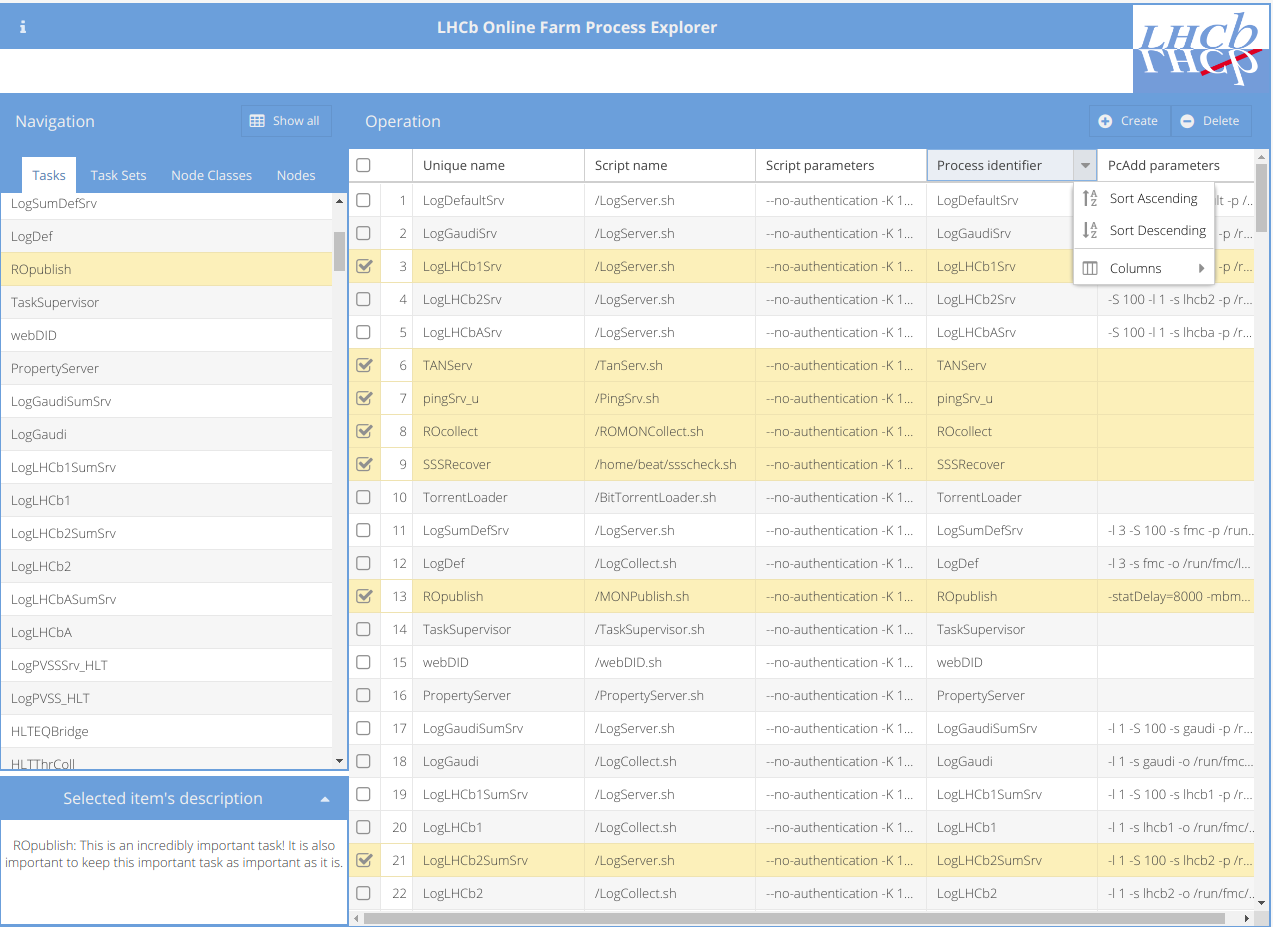
\includegraphics[scale=0.35]{images/gui.png}
    \caption{An outlook of the graphical user interface}
    \label{fig:gui}
\end{figure}

\noindent
By no means was the development easy. It was a great opportunity for a summer student to improve programming skills and get to know a new development framework relatively well.

%==============================================
%           Derived applications
%==============================================

\section{Derived applications}
\hspace{0.6cm}

The derived applications are all of the programs that do not qualify as back-end (server side) or front-end (client side) solutions but still utilize the data provided by the database, through the Main API.

%==============================================

\subsection{New boot script}
\hspace{0.6cm}

To fully recreate the functionality of the previous solution, a new boot script had been written. As a modular structure of the system has been introduced, the boot script is no longer responsible for both storage and execution of the configuration data - it is just an optional client application for the Main API. The inner structure of the script is thus very simple - it just uses Main API's methods to find all tasks that belong to a specific node regular expression (input).

%==============================================

\subsection{Unit testing script}
\hspace{0.6cm}

In the IT world, unit testing is a name for validation of the program's functionality. In the designed system, the most critical part that needed testing in order to go into production (replace the old solution) was naturally the Main API. This subsystem is used to check if the changes made to the API do not harm its functionality.
\newline

\noindent
Unit testing was surely not the most exciting part of the project. In principle, the script had to execute all possible API methods and verify if they work properly. To achieve that, the script first verifies the API's response to the method call and then checks if the requested action had modified the underlying database in the right way.
\newline  \newline
This description applies not only to the correctly called methods (all of the parameters provided, no logical errors). The unit testing script also needs to verify if all of the possible errors are handled correctly - right error code is returned and no modifications are made to the database.
\newline  \newline
After each test method call, the script prompts the result in the command line using unified formatting and font colouring - it is easy to spot an error and find its source. It also returns the number of errors found - it is possible to integrate the script in a larger production unit testing system.

%==============================================
%           Prize
%==============================================

\section{Moritz Karbach summer student prize 2018 winner}
\hspace{0.6cm}

This summer student project has been awarded with 2018 Moritz Karbach prize which is a collaboration award given to summer students "as recognition for outstanding performance" annually, in memory of Moritz Karbach, a young LHCb physicist who lost his life in a climbing accident in April 2015.
\newline

\noindent
To be qualified for the prize, the students had to give a brief (10 minutes + 5 minutes for questions) presentation of their projects and sum up their work in CERN (after roughly two out of three months of their stay). More details about the criteria of the award and a list of the winners from previous years (along with the presentations of the projects) can be found under the following link:
\newline

\noindent\fcolorbox{logocolor}{white}{%
    \parbox{\textwidth}{%
        \centering
        \href{https://lhcb.web.cern.ch/lhcb/Collaboration_prizes/Moritz_Karbach_summer_student_prize.html}{The Moritz Karbach summer student prize (LINK)}. 
    }%
}
\vspace{0.6cm}

\begin{figure}[H]
\centering
    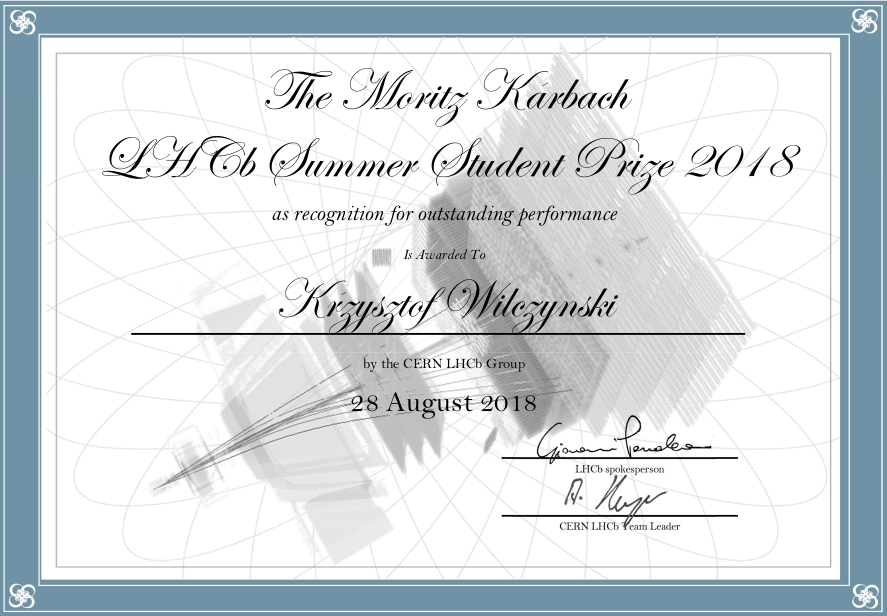
\includegraphics[scale=0.42]{images/Certificate.png}
    \caption{The Moritz Karbach prize diploma}
    \label{fig:diploma}
\end{figure}

\begin{figure}[H]
\centering
    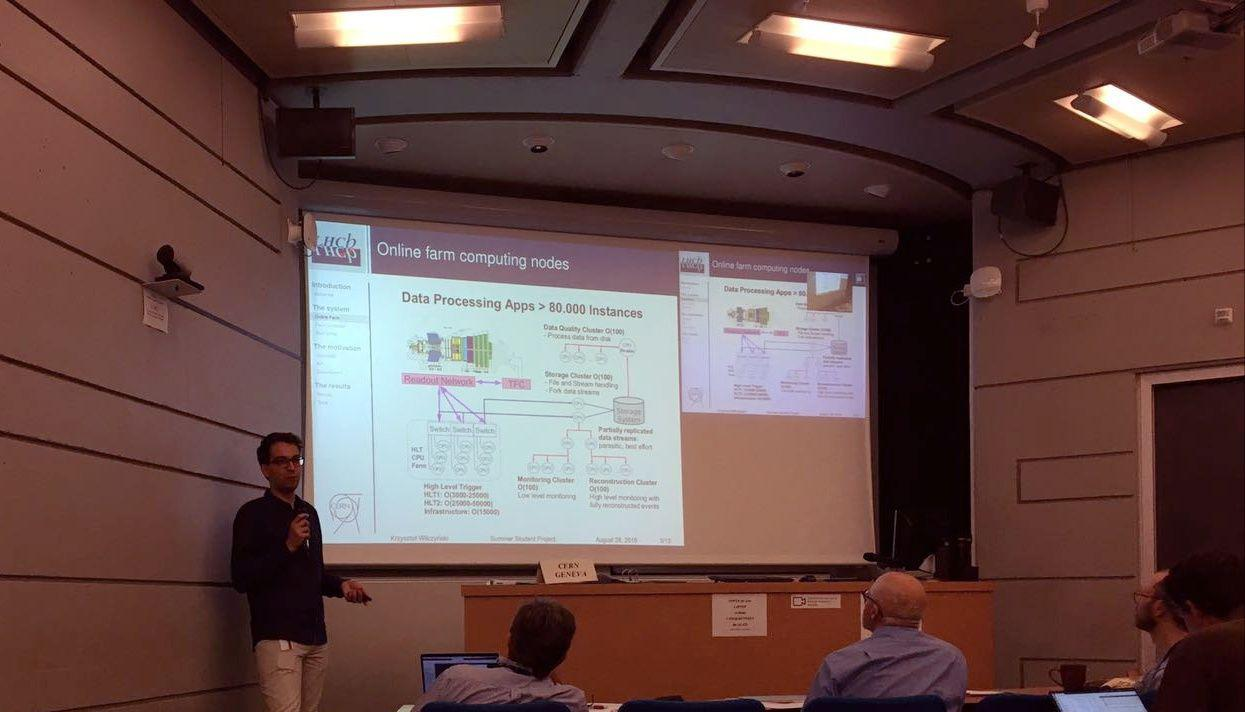
\includegraphics[scale=0.4]{images/Project_Presentation.jpg}
    \caption{A photo from the presentations session}
    \label{fig:presentation}
\end{figure}

%==============================================
%           Summary
%==============================================

\newpage
\section{Summary}
\hspace{0.6cm}


By using the described data-driven solution, it will be a lot more convenient to review, modify and diagnose the configuration of the tasks running on the Online farm nodes. The software is obeying modern development standards that make it flexible and future-proof. 
Unlike its predecessor, the new system can handle rapid growth of CPU number in the future upgrades of the LHCb detector while not making the maintaining, debugging, modification and testing incredibly complex.
\newline

\noindent
All of the project's goals have been successfully achieved and the system will be deployed in the production environment - the LHCb Online farm. The summer student has built and tested functional prototypes of each part of the solution which will be maintained and improved further by project supervisor - Markus Frank. 
\newline

\noindent
The summer student project in LHCb Online group was a great opportunity to develop programming skills under guidance of immensely experienced supervisor while attending lectures covering various topics ranging from particle physics, through computing, to accelerator engineering. The lectures, together with numerous visits in research facilities, fascinating workshops and the applied project made up the best, horizon-broadening summer a curious student could dream of. 
\newline  \newline
The Summer Student Programme was indeed an experience like nowhere else on Earth.
\vspace{3cm}

\centerline{\underline{\textbf{Thank You, CERN!}}}
\vspace{3cm}


% Include or exclude the appendix - for the HR department

%==============================================
%           Appendix
%==============================================

\newpage
\section{Appendix}

\subsection{Code repositories}
\hspace{0.6cm}

The developed software (and some technical documentation) can be found in a Bitbucket repository linked below.
\newline

\noindent\fcolorbox{logocolor}{white}{%
    \parbox{\textwidth}{%
        \centering
        \href{https://bitbucket.org/3sztof/lhcb_online/src/master/}{The author's open-source code repository (LINK)}. 
    }%
}

\vspace{0.6cm}

\noindent
In the future, the project will be maintained by the main supervisor - Markus Frank. The official, production repository can be found here:
\newline

\noindent\fcolorbox{logocolor}{white}{%
    \parbox{\textwidth}{%
        \centering
        \href{https://gitlab.cern.ch/lhcb/OnlineExtra/tree/master/Online/TaskDB}{The project maintained by Markus Frank in LHCb Gitlab repository (LINK)}. 
    }%
}
\vspace{0.6cm}


%==============================================

\subsection{Database}
\hspace{0.6cm}

A schema of the database tables and their columns recreating the task $\xleftrightarrow{}$ task set $\xleftrightarrow{}$ node class $\xleftrightarrow{}$ node hierarchy is shown in figure \ref{fig:schema}.
\newline

\begin{figure}[H]
\centering
    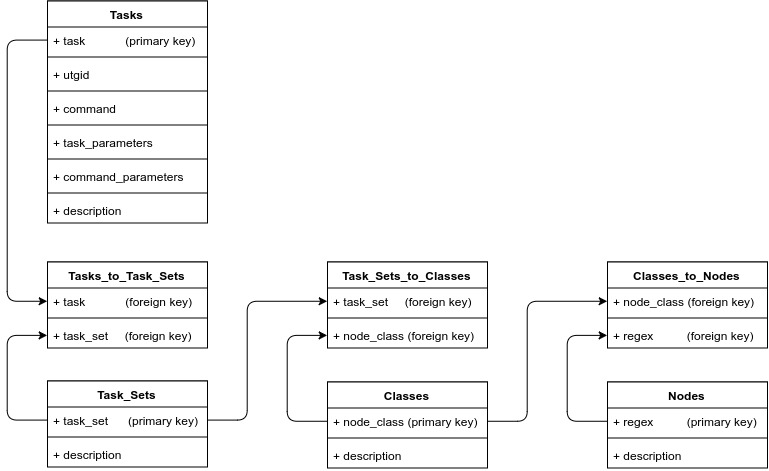
\includegraphics[scale=0.58]{images/Database_Schema.jpg}
    \caption{Database schema diagram}
    \label{fig:schema}
\end{figure}

\newpage
\noindent
To maintain the relationships between the "parent" and "child" data in the hierarchy, it was required to introduce the following three additional tables:

\begin{multicols}{3}
    \begin{itemize}
        \item Tasks\_to\_Task\_Sets
        \item Task\_Sets\_to\_Classes
        \item Classes\_to\_Nodes
    \end{itemize}
\end{multicols}

\noindent
Those three structures contain pairs of assignments that allow the creation of "many to many" relationships between the primary keys (unique names) of the assigned items and their parent tables. For example, one task can belong to many tasks sets while one task set can contain many tasks. 
\newline

%==============================================

\noindent
The arrows visible on figure \ref{fig:schema} were meant to visualize the constraints that were put on the data entries. Besides the "unique" primary keys, the database utilizes "foreign key" mechanism that was needed to introduce many to many relationship between the tables of sets and items assigned to the sets. 
\newline

\noindent
The behaviour of data referenced to as a "foreign key" has to be defined in case the primary key it references is deleted or updated. In the current solution, two events were defined:

\begin{itemize}
    \item On update cascade \\ (update the foreign key if the original value was updated in its mother table)
    \item On delete cascade \\ (delete the foreign key if the original value was deleted from its mother table)
\end{itemize}

%==============================================

\noindent
The database engine used in the current solution is SQLite as it is an integral part of both Python 2.7 and Python 3 - this way no maintaining is needed after software upgrade, the dependencies should be kept safe.
\newline

\noindent
While most of the early python scripts used sqlite3 Python module to connect to the database, the final Main API script utilizes sqlalchemy (foreign module) as it allows for easier transition to other database engines (relational) should the situation demand it in the future. Sqlalchemy connection and query objects are compatible with the database engines such as SQLite, Postgresql, MySQL, Oracle, MS-SQL, Firebird, Sybase and many others.

%==============================================

\subsection{Main API methods}
\hspace{0.6cm}

The Main API methods were implemented as methods of a Python class named "TaskDB". The following points contain their brief descriptions and sample method calls. Note that the parameters of the example calls put in angle brackets, like "<key>" are mandatory and specifying their key name is optional (they can be passed just as a value in the correct order), the others are optional.  


\newpage
\begin{itemize}
    % Add
    \item 
        \textbf{addItem} (where "Item" should be replaced with "Task", "TaskSet", "Class" or "Node"): creates a new entry in the specified Item's table. The required value is the table's primary key (see figure \ref{fig:schema}). Note that specifying only the primary key is not enough for a Task configuration to be considered complete: in order for it to work correctly, at least "utgid" and "command" values (required by pcAdd) should also be specified.

        \begin{sexylisting}[colback=white]{addItem method call}
TaskDB.addTask(<task>="SampleTask",
               utgid="UserDefinedIdentifier",
               command="sleep.sh",
               command_parameters="-t 3",
               description="Sleep for 3 seconds")
        \end{sexylisting}
    
    % Delete
    \item 
        \textbf{deleteItem} (where "Item" should be replaced with "Task", "TaskSet", "Class" or "Node"): deletes an entry from the specified Item's table. The only (and required) parameter of this method is Item's primary key (unique name). Note that when deleting an entry this way, all of its foreign key dependencies will also be deleted.
        
        \begin{sexylisting}[colback=white]{deleteItem method call}
TaskDB.deleteTask(<task>="SampleTask")
        \end{sexylisting}
    
    % Modify
    \item 
        \textbf{modifyItem} (where "Item" should be replaced with "Task", "TaskSet", "Class" or "Node"): modifies the specified Item's data when given correct keys and values, or leaves them unchanged otherwise.
        \begin{sexylisting}[colback=white]{modifyItem method call}
TaskDB.modifyTask(<original_task>="SampleTask",
                  task="ModifiedTask", 
                  description="This task was modified")
        \end{sexylisting}
    
    % Get
    \item 
        \textbf{getItem} (where "Item" should be replaced with "Task", "TaskSet", "Class" or "Node"): returns a JSON object containing all of the Item's data (in "data" root value array). If no argument is specified, or "*" is provided, the method will return (by default) all of the Items of given type.
        \begin{sexylisting}[colback=white]{getItem method call}
TaskDB.getTask(<task>="SampleTask")
        \end{sexylisting}
        \begin{sexylisting}[colback=white]{getItem response}
{"data":[
    {
        "task": "SampleTask",
        "description": "Sample task's description
    }
]}
        \end{sexylisting}
    
    % Assign
    \item 
        \textbf{assignItem} (where "Item" should be replaced with "Task", "TaskSet" or "Class"): assigns the specified Item to its parent. Two parameters are required: one pointing to the primary key of the child (item to be assigned) and the other pointing to the primary key of an existing set.
        \begin{sexylisting}[colback=white]{assignItem method call}
TaskDB.assignTask(<task>="SampleTask", 
                  <task_set>="SampleTaskSet")
        \end{sexylisting}
        \begin{sexylisting}[colback=white]{assignItem method call}
TaskDB.assignClass(<node_class>="SampleNodeClass", 
                   <regex>="SampleNodeRegex")
        \end{sexylisting}
        
    % Unassign
    \item 
        \textbf{unassignItem} (where "Item" should be replaced with "Task", "TaskSet" or "Class"): unassigns the specified Item from its parent. Two parameters are required: one pointing to the primary key of the child (item to be unassigned) and the other pointing to the primary key of an existing set.
        \begin{sexylisting}[colback=white]{unassignItem method call}
TaskDB.unassignTask(<task>="SampleTask", 
                    <task_set>="SampleTaskSet")
        \end{sexylisting}
        \begin{sexylisting}[colback=white]{unassignItem method call}
TaskDB.unassignClass(<node_class>="SampleNodeClass", 
                     <regex>="SampleNodeRegex")
        \end{sexylisting}
      
\newpage  
    % InSet
    \item
        \textbf{itemsInSet} (where "items" should be replaced with "tasks", "tasksets" or "nodeclass" and "Set" should be replaced with "Set", "Class" or "Node" accordingly): returns a JSON object containing all of the items assigned to a given set. The only required parameter is the Set's primary key (unique name).
        \begin{sexylisting}[colback=white]{itemsInSet method call}
TaskDB.tasksetsInClass(<node_class>="SampleNodeClass")
        \end{sexylisting}
        \begin{sexylisting}[colback=white]{itemsInSet response}
{"data":[
    {
        "task_set": "SampleTaskSet",
    },
    {
        "task_set": "AnotherSampleTaskSet"
    }
]}
        \end{sexylisting}
        
    % GetTasksByNode
    \item
        \textbf{getTasksByNode}: returns all of the tasks that should be started on a specified node (regular expression) in a form of an array. If "*" is provided as an argument, the method will return all of the tasks that are assigned to all of the existing nodes.
        \begin{sexylisting}[colback=white]{getTasksByNode method call}
TaskDB.getTasksByNode(<node>="*")
        \end{sexylisting}
        
        % Edit the above (update after changes in the API)
        
\end{itemize}


%Something about other Classes in the script? Connection?


%==============================================

\subsection{Front-end connectors}
\hspace{0.6cm}

In the latest version of the system, both JSONRPC and XMLRPC protocols can be used to interact with the Main API using the POST HTTP method and JSON/XML request body. The following call and response examples aim to show a similarity between the two protocols and deepen the reader's understanding of what is happening in the back-end $\xleftrightarrow{}$ front-end communication layer.

\newpage
\begin{itemize}
    \item 
        JSONRPC
        \begin{sexylisting}[colback=white]{JSONRPC request body}
{
    "jsonrpc": "2.0", 
    "method": "getSet", 
    "params": {"task_set": "SampleSet"}, 
    "id": 3
}
        \end{sexylisting}
        \begin{sexylisting}[colback=white]{JSONRPC response body}
{
    "jsonrpc": "2.0",
    "result":
        [
            {
                "task_set": "SampleSet", 
                "description": "Description"
            }       
        ],
    "id": 3
}
        \end{sexylisting}
    \item
        XMLRPC
        \begin{sexylisting}[colback=white]{XMLRPC request body}
<?xml version='1.0'?> 
<methodCall>
    <methodName>getSet</methodName>\n 
    <params>
    <param>
        <value><struct>
        <member>
            <name>task_set</name>
            <value><string>SampleSet</string></value>
        </member>
        </struct></value>
    </param>
    </params>
</methodCall>
        \end{sexylisting}
        \begin{sexylisting}[colback=white]{XMLRPC response body}
<?xml version='1.0'?>
<methodResponse>
    <params>
    <param>
        <value><array><data>
        <value><struct>
        <member>
            <name>task_set</name>
            <value><string>SampleSet</string></value>
        </member>
        <member>
            <name>description</name>
            <value><string>Description</string></value>
        </member>
        </struct></value>
        </data></array></value>
    </param>
    </params>
</methodResponse>
        \end{sexylisting}
\end{itemize}

\noindent
The links below point to the specifications of JSONRPC and XMLRPC protocols, should the reader be interested in more advanced features.
\newline

\noindent\fcolorbox{logocolor}{white}{%
    \parbox{\textwidth}{%
        \centering
        \href{https://www.jsonrpc.org/specification}{JSONRPC protocol specification (LINK)}. 
    }%
}
\newline

\noindent\fcolorbox{logocolor}{white}{%
    \parbox{\textwidth}{%
        \centering
        \href{http://xmlrpc.scripting.com/spec.html}{XMLRPC protocol specification (LINK)}. 
    }%
}

%==============================================

%\subsection{Command line interface}
%\hspace{0.6cm}

%aa

%==============================================

\subsection{Sencha CMD tool}
\hspace{0.6cm}

The Sencha Ext JS application (graphical front-end) was submitted to the repository in a minimized form - the complete build directory contained over 25000 automatically generated files and was taking over 370 MB of disk space. All of those dependencies are only required to run the debugging and the development server, most of them were belonging to Ext JS SDK (GPL, version 6.2.0).
\newline

\noindent
While the full structure of the development folder is not needed for simple deployment of the application, it might be required to fix some bugs or extend its functionality in the future. For this, one needs to regenerate the development environment using Sencha CMD tool.

\newpage
\noindent
The tools needed for environment regeneration are:
\newline

\noindent\fcolorbox{logocolor}{white}{%
\parbox{\textwidth}{%
    \centering
    \href{https://www.sencha.com/products/extjs/cmd-download/}{Sencha CMD tool (LINK) \\ (v6.6.0.13 has been used during the application development)}  
    }%
}
\vspace{0.3cm}

\noindent\fcolorbox{logocolor}{white}{%
\parbox{\textwidth}{%
    \centering
    \href{https://www.sencha.com/legal/gpl/}{Sencha Ext JS SDK, GPL (LINK) \\ (v6.2.0 has been used during the application development)}  
    }%
}
\newline

\noindent
To build the application from the source, the following actions are needed:

\begin{itemize}
    \item
        Modify the workspace.json file to specify path to the Sencha Ext JS SDK directory. The version is an optional parameter that should be changed in case of SDK version upgrade. The workspace.json file fragment indicating this path should look like this:
        \begin{sexylisting}[colback=white]{workspace.json for fast building}
"frameworks": {
    "ext": {
        "path":"/home/einstein/ext-6.2.0",
        "version":"6.2.0.981"
    }
}
        \end{sexylisting}
        
    \item
        Generate a sample Ext JS application to recreate the build environment by running the command provided in the following code example outside the application's root folder:
        \begin{sexylisting}[colback=white]{environment regeneration}
>mkdir temp
>sencha -sdk /home/einstein/ext-6.2.0 generate app
 MyApp temp
        \end{sexylisting}
        Then, recursively copy (cp -r) the hidden ".sencha/" directory from the sample application's directory (temp) to the root directory of the original project.
        
    \item
        In the application's root directory, run the command provided in the next code example to build the application in "./build/<type>/LHCb".
        \begin{sexylisting}[colback=white]{application building}
>sencha app build (defaults to production build)
>sencha app build testing (more logging in JS console)
        \end{sexylisting}
\end{itemize}

\noindent
The application built this way should be ready to be deployed on an Apache server with proxy routing to the back-end services on the same port (or the development file/service server provided in the TaskDB folder).

\noindent
To run the application in exhaustively debugging mode (a server provided by Sencha CMD tool, on port 1841, which constantly updates the hosted file system - continuous building), one needs to take the following steps:

\begin{itemize}
    \item
         Modify the workspace.json file to specify path to a minimized SDK copy in the application's root directory. The version is an optional parameter that should be changed in case of SDK version upgrade. The workspace.json file fragment indicating this path should look exactly like this:
        \begin{sexylisting}[colback=white]{workspace.json for debug building}
"frameworks": {
    "ext": {
        "path":"ext",
        "version":"6.2.0.981"
    }
}
        \end{sexylisting}
    \item
        Generate a sample Ext JS application to recreate the build environment by running the command provided in the following code example outside the application's root folder:
        \begin{sexylisting}[colback=white]{environment regeneration}
>mkdir temp
>sencha -sdk /home/einstein/ext-6.2.0 generate app
 MyApp temp
        \end{sexylisting}
        Then, recursively copy (cp -r) the hidden ".sencha/" and "ext/" directories from the sample application's directory (temp) to the root directory of the original project.
    \item
        In the application's root directory, run the command provided in the next code example to deploy the debugging server on local port 1841.
        \begin{sexylisting}[colback=white]{starting the debug server}
>sencha app watch
        \end{sexylisting}
\end{itemize}

\newpage

\noindent
The Sencha CMD tool can also be used to upgrade the application to newer versions of Ext JS SDK (GPL) should the situation demand it in the future. This can be achieved by simply running the command provided in the next code example in the application's root directory.

\begin{sexylisting}[colback=white]{starting the debug server}
>sencha app upgrade [path to updated framework]
\end{sexylisting}

\noindent
Please be warned that this operation might require further changes if customization has been applied to the automatically generated files. For more details on the upgrade function of Sencha CMD tool, consult the guide linked below.
\newline

\noindent
\fcolorbox{logocolor}{white}{%
\parbox{\textwidth}{%
    \centering
    \href{https://docs.sencha.com/cmd/guides/cmd_upgrade.html}{Sencha CMD tool upgrade operation (LINK)}  
    }%
}










\begin{comment}

%-------------- Examples ----------------------

\newpage
\section{Examples}

Examples

%----------- Insert image ---------------------

\insererfigure{logos/cern.png}{3cm}{Caption}{Label}

% \begin{figure}[H]
%     	\centering
%     	
\includegraphics[scale=0.1]{warsaw1.png}
%     	%\caption{Wykresy Bodego transmitancji G, HG oraz HGW}
%     	%\label{fig:transmitancja}
% \end{figure}

Cite the image number: \ref{fig: Label}


%------------- Equation ------------------------

\begin{equation} \label{eq: exemple}
\rho + \Delta = 42
\end{equation}

Equation number reference: \ref{eq: exemple}

% ---------- Math in text ----------------------

Blablabla \$ blablabla $\rho$. 

\end{comment}

\end{document}

